\documentclass[11pt,a4paper,oneside]{article}
\usepackage[utf8]{inputenc}
\usepackage[french]{babel}
\usepackage[T1]{fontenc}
\usepackage{graphicx}

\usepackage{sectsty}
\usepackage{xcolor}
%\definecolor{couleur_section}{RGB}{0,0,128} % Cette nouvelle couleur s'appelle "couleur_section", que nous utiliserons pour les titres de type "section"
%\sectionfont{\color{couleur_section}}
\subsubsectionfont{\itshape}

\usepackage{charter}
\usepackage{hyperref}
\usepackage{listings}
\usepackage{wrapfig}

\usepackage[left=2cm,right=2cm,top=2cm,bottom=2cm]{geometry}
\setlength{\headheight}{15pt}
\usepackage{fancyhdr}
\pagestyle{fancy}
\usepackage{lastpage}
\fancyhf{}
\renewcommand\headrulewidth{0pt}
%\fancyhead[L]{Dossier Technique}
\renewcommand\footrulewidth{1pt}
\fancyfoot[C]{\textbf{Page \thepage/\pageref{LastPage}}}
\author{Mylann Dupuy}
\title{Dossier Technique}
\date{30 Mars 2019 - Version 2.0}

\setlength{\parindent}{0cm}
\setlength{\parskip}{1ex plus 0.5ex minus 0.2ex}
\newcommand{\hsp}{\hspace{20pt}}
\newcommand{\HRule}{\rule{\linewidth}{0.5mm}}
\begin{document}

\begin{titlepage}
  \begin{sffamily}
  \begin{center}

    \textsc{\LARGE Dossier Technique de la période professionnelle}\\[6.5cm]
    
\includegraphics[scale=1]{Ressources/polysoude.jpg}
    % Title
        \HRule \\[0.4cm]
        { \huge \bfseries TECHNICIEN SUPÉRIEUR DE SUPPORT INFORMATIQUE\\[0.4cm] }
        \HRule \\[6.5cm]

    % Author and supervisor
    \begin{minipage}{0.4\textwidth}
      \begin{flushleft} \large
        Candidat : Mylann \textsc{Dupuy}\\
        Promotion : HAPPT201\\
        Titre : T2SI
      \end{flushleft}
    \end{minipage}
    \begin{minipage}{0.5\textwidth}
      \begin{flushright} \large
        \emph{Tuteur :} M. Olivier \textsc{Naud}\\
        \emph{Binôme :} M. Antoine \textsc{Etrillard}\\
      \end{flushright}
    \end{minipage}

    \vfill

    % Bottom of the page
    {\large Version 2.3 - 16 Mai 2019}

  \end{center}
  \end{sffamily}
\end{titlepage}
\newpage

% ##### Page 3 #####
\tableofcontents
\newpage
\setcounter{page}{2}
\newpage

% ##### Page 5 #####
\section*{Introduction}
\addcontentsline{toc}{section}{Introduction}
Avant de parler de moi, je souhaiterais tout d’abord remercier l’entreprise \textbf{POLYSOUDE} ainsi que l'équipe informatique qui m’a accueilli depuis \textbf{Septembre 2017} au sein de leur service.

\subsection*{Mon parcours}
Suite à l’obtention d’un \textbf{BAC PRO SEN} (Systèmes Électroniques Numériques) d'un lycée professionnel au Mans (72), j’ai ensuite débuté un \textbf{BTS SIO} avant de m’orienter vers un l'\textbf{ENI} depuis septembre 2017 pour le titre \textbf{BAC +2 T2SI} sous la forme d'une formation en alternance.

\subsection*{Pourquoi cette formation et pas une autre ?}

C'est en recherchant une nouvelle formation que j'ai découvert l'existence du centre de formation de l'\textbf{ENI}.\\

Mon intérêt s’est porté sur la \textbf{formation T2SI} (qui m'était inconnue à ce jour).Cette dernière se rapprochant, au niveau du contenu, du BTS SIO mais avec une approche beaucoup plus technique et plus proche de mes attentes. \\
\\
L’objectif que je me suis fixé après avoir été retenu pour cette formation est de décrocher le titre afin d’intégrer une entreprise avec des possibilités d’évolutions futures.\\
Cela me permettrait ainsi de renouveler et de faire évoluer mes connaissances et ce dans le cadre d’un travail en équipe.
\newpage

% ##### Page 4 #####
\section{Présentation de l'entreprise}
L'entreprise POLYSOUDE a été fondée en 1961 en présentant comme "pionnière dans la conception et la fabrication de matériel de soudage orbital". En 58 ans d'existence, l'entreprise a ouverte diverses filiales à travers le monde.\\

Aujourd'hui, la maison mère de POLYSOUDE basée à Nantes compte 200 employés à son actif ainsi que 12 filiales / bureaux sans oublier les partenaires à travers le monde (+ de 50 partenaires). \\

Toutes les informations concernant POLYSOUDE sont disponible ici : \textbf{\hyperlink{https://www.polysoude.com/}{www.polysoude.com}}

\subsection{Hiérarchie}
L’organigramme ci-dessous présente l’organisation des différents départements et services de Polysoude.
\begin{figure}[h!]
  \centering
  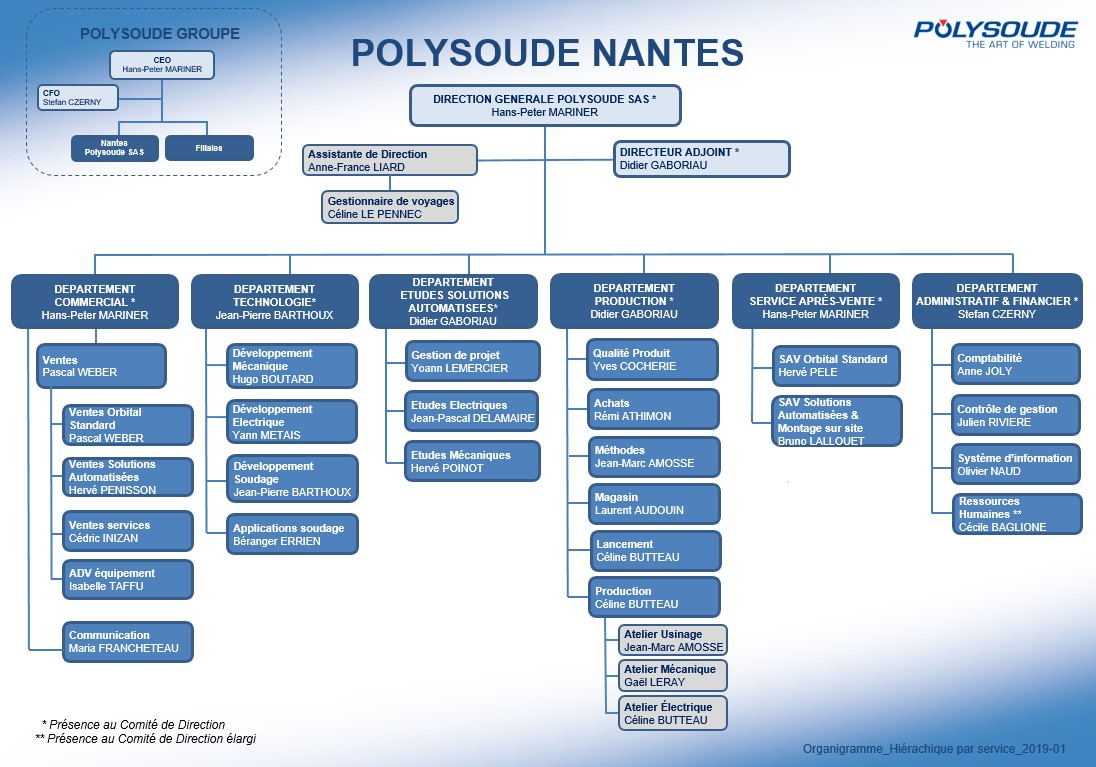
\includegraphics[width=\linewidth]{Ressources/Organigramme.jpg}
  \caption{Organigramme}
\end{figure}

Dans mon cas, mon collègue, \textbf{Antoine ETRILLARD}, et moi-même sommes sous la responsabilité d'\textbf{Olivier NAUD}, Responsable du Service Informatique (RSI), lui-même sous la responsabilité de  \textbf{Stefan CZERNY}, Directeur du département Administratif \& Financier.
\newpage

% ##### Page 5 #####
\section{Présentation de l'informatique dans l'entreprise}
\subsection{L'équipe}
Avant de parler de l’infrastructure, je vais vous présenter les membres qui composent l’ensemble du service IT, chaque collaborateur ayant un rôle à jouer que ce soit pour les logiciels métiers ou pour l’assistance aux utilisateurs.

\begin{itemize}
    \item \textbf{Olivier NAUD :} Le responsable du Service IT s'occupe principalement de l'administration système et réseau de l'entreprise (Gestion des droits O365, Infra, Téléphonie, etc...) avec l'aide de diverses prestataires. \\
    %%%%%%%%%%
    \item \textbf{Vanessa PELLE :} Responsable de l'ERP \footnote{Enterprise Resource Planning} nommé \hyperlink{https://www.ifsworld.com/fr/}{IFS}. Met en place et développe  différents modules et outils, forme les utilisateurs, traite les incidents et les demandes liées. \\
    %%%%%%%%%%
    \item \textbf{Maxime CLAVIER :} Ce collaborateur s’occupe principalement du logiciel de gestion des données techniques (PDM), via la solution proposée par \hyperlink{https://www.solidworks.com/fr}{SOLIDWORKS} \footnote{Logiciel de conception CAO 3D} ainsi que du logiciel de gestion des planning \hyperlink{https://www.visual-planning.com/fr/}{VISUAL PLANNING  (VP)}. Forme et assiste les collaborateurs sur l’utilisation de ces applications.\\
    %%%%%%%%%%
    \item \textbf{Antoine ETTRILLARD :} 1\ier{} pilier du service IT, il traite les demandes d'appels / mails en créant les tickets GLPI \footnote{Gestion Libre de Parc Informatique} puis assiste les utilisateurs pour la résolution de leur(s) problème(s) et/ou demande(s).
\end{itemize}
   
\subsection{Matériels}
L'infrastructure est gérée en interne, je m'explique :

\begin{itemize}
    \item \textbf{Serveurs :} Qu'ils soient physiques ou virtuels (sous un hyperviseur de type 1 : \textbf{Hyper-V)}, ils sont gérés par notre responsable et sous contrat chez différents prestataires / revendeurs. Tout les serveurs sont basés sur Windows Server (2003, 2008, 2012 R2).\\
    %%%%%%%%%%
    \item \textbf{Clients :}Les collaborateurs de l’entreprise utilisent tous des machines physiques (postes fixes ou portables). Une liste exhaustive des différentes machines utilisées est présentée plus bas (Points 2.2.1 et 2.2.2). Les postes clients fonctionnent sous Windows 7 ou Windows 10. \\
\end{itemize}
L’ensemble des serveurs présents dans l’entreprise sont dupliqués vers un site distant (Data Center) dans le cadre du PRA (Plan de Reprise d’Activité).

Les données sont également sauvegardées périodiquement.
    
Dû à la limite de page imposée pour ce dossier, je ne parlerai que des postes clients.
\newpage

% Type matériel réel / Virtuel
\subsubsection{Postes Fixes}
% ### 1 ###
\begin{wrapfigure}{c}{7cm}
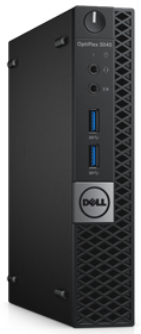
\includegraphics[scale=0.4]{Ressources/Materiel/3040.png}\vspace{-2cm}
\end{wrapfigure}
\paragraph{}\textbf{Dell OptiPlex 3040 Micro :} \\
\begin{itemize}
\item \textbf{CPU :} Intel Core i3
\item \textbf{RAM :} 8 Go
\item \textbf{OS :} Windows 7 / Windows 10
\item \textbf{Disque Dur :} 256 Go SDD / 500 Go HDD
\item \textbf{Quantité :} 41 unités
\\ \\ \\ \\
\end{itemize}
%%%%%%%%%%%%%%%
\begin{wrapfigure}{c}{7cm}
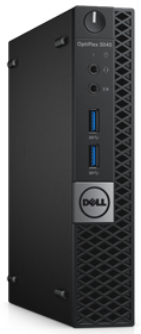
\includegraphics[scale=0.4]{Ressources/Materiel/3040.png}\vspace{-2cm}
\end{wrapfigure}
\paragraph{}\textbf{Dell Optiplex 3050 Micro :} \\
\begin{itemize}
\item \textbf{CPU :} Intel Core i5-7500T // Intel Core i3-7100T
\item \textbf{RAM :} 8 Go
\item \textbf{OS :} Windows 7 / Windows 10
\item \textbf{Disque Dur :} 256 Go SSD // 500 Go HDD
\item \textbf{Quantité :} 2 unités
\\ \\ \\ \\
\end{itemize}
%%%%%%%%%%%%%%%
\begin{wrapfigure}{c}{7cm}
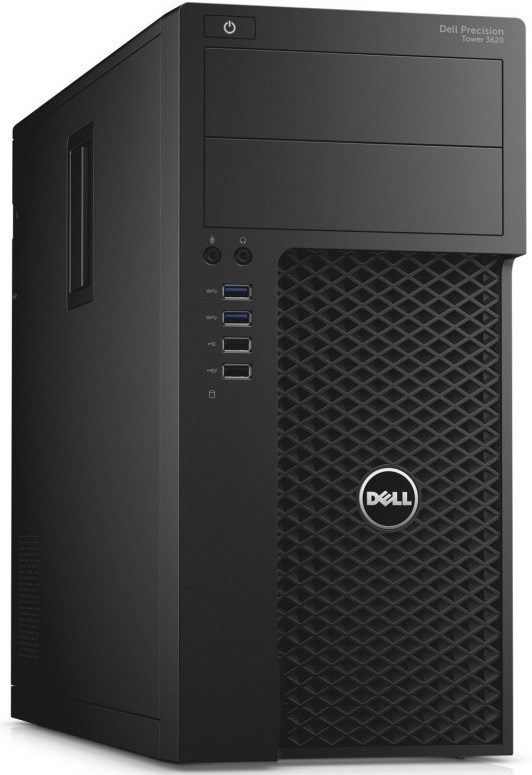
\includegraphics[scale=0.3]{Ressources/Materiel/3620.jpg}\vspace{-2cm}
\end{wrapfigure}
\paragraph{}\textbf{Dell Precision 3620 :} \\
\begin{itemize}
\item \textbf{CPU :} Intel Core i7-6700
\item \textbf{RAM :} 8 Go
\item \textbf{OS :} Windows 7 // Windows 10
\item \textbf{Disque Dur :} 256 Go SSD // 500 Go SSHD
\item \textbf{Quantité :} 12 unités
\\ \\ \\ \\
\end{itemize}
\newpage

\subsubsection{Postes Portables}
% ### 2 ###
\begin{wrapfigure}{c}{7cm}
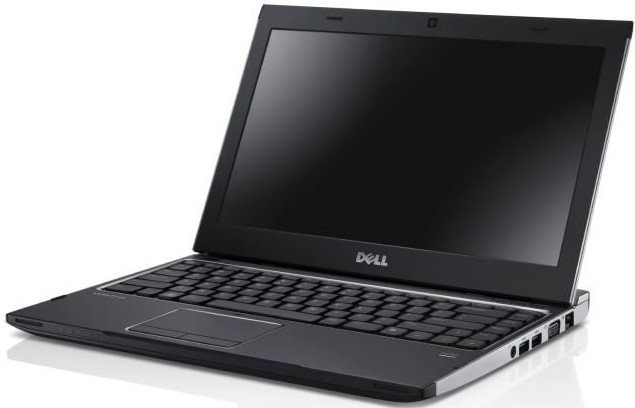
\includegraphics[scale=0.4]{Ressources/Materiel/V131.jpg}\vspace{-2cm}
\end{wrapfigure}
\paragraph{}\textbf{Dell Vostro V131 :} \\
\begin{itemize}
\item \textbf{CPU :} Intel Core i5-2450M
\item \textbf{RAM :} 8 Go
\item \textbf{OS :} Windows 7
\item \textbf{Disque Dur :} 500 Go HDD
\item \textbf{Quantité :} 13 unités
\\ \\ \\ \\
\end{itemize}
%%%%%%%%%%%%%%%
\begin{wrapfigure}{c}{7cm}
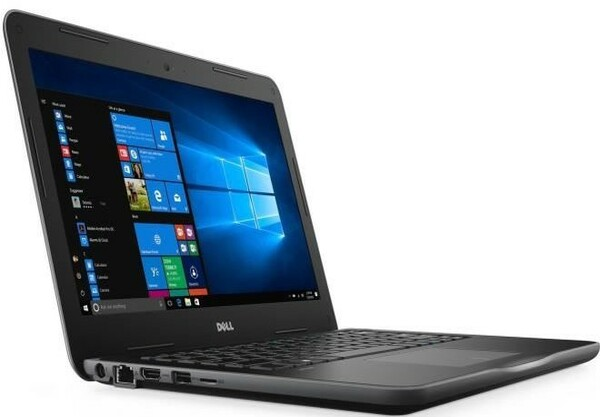
\includegraphics[scale=0.4]{Ressources/Materiel/L3380.jpg}\vspace{-2cm}
\end{wrapfigure}
\paragraph{}\textbf{Dell Latitude 3380 :} \\
\begin{itemize}
\item \textbf{CPU :} Intel Core i5-7200U
\item \textbf{RAM :} 8 Go
\item \textbf{OS :} Windows 7
\item \textbf{Disque Dur :} 256 Go SSD / 500 Go HDD
\item \textbf{Quantité :} 17 unités
\\ \\ \\ \\
\end{itemize}
%%%%%%%%%%%%%%%
\begin{wrapfigure}{c}{7cm}
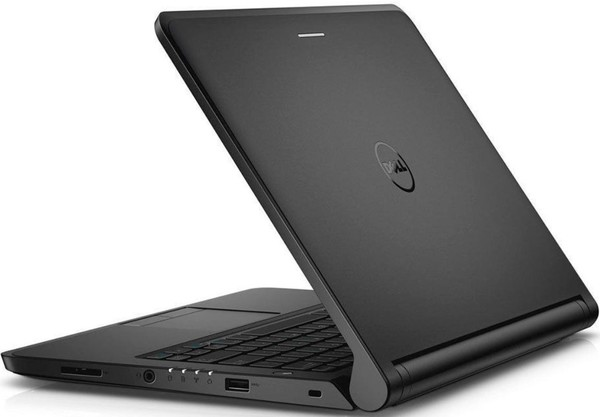
\includegraphics[scale=0.4]{Ressources/Materiel/L3350.jpg}\vspace{-2cm}
\end{wrapfigure}
\paragraph{}\textbf{Dell Latitude 3350 :} \\
\begin{itemize}
\item \textbf{CPU :} Intel Core i5-4210U
\item \textbf{RAM :} 8 Go
\item \textbf{OS :} Windows 10
\item \textbf{Disque Dur :} 256 Go SSD
\item \textbf{Quantité :} 14 unités
\\ \\ \\ \\
\end{itemize}
%%%%%%%%%%%%%%%
\begin{wrapfigure}{c}{7cm}
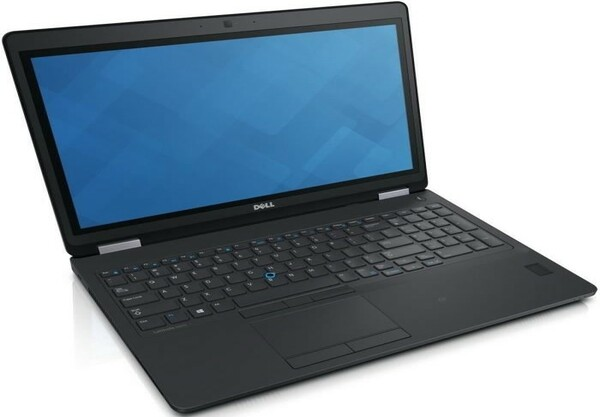
\includegraphics[scale=0.4]{Ressources/Materiel/LE5570.jpg}\vspace{-2cm}
\end{wrapfigure}
\paragraph{}\textbf{Dell Latitude E5570 :} \\
\begin{itemize}
\item \textbf{CPU :} Intel Core i7-6820HQ
\item \textbf{RAM :} 8 Go
\item \textbf{OS :} Windows 10
\item \textbf{Disque Dur :} 256 Go SSD
\item \textbf{Quantité :} 4 unités
\\ \\ \\ \\
\end{itemize}
%%%%%%%%%%%%%%%
\begin{wrapfigure}{c}{7cm}
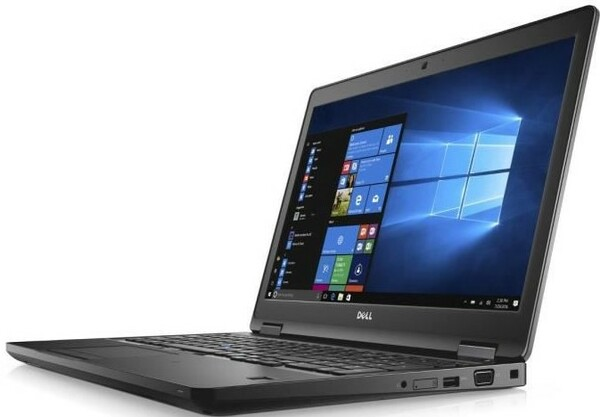
\includegraphics[scale=0.4]{Ressources/Materiel/L5580.jpg}\vspace{-2cm}
\end{wrapfigure}
\paragraph{}\textbf{Dell Latitude 5580 :} \\
\begin{itemize}
\item \textbf{CPU :} Intel Core i7-6820HQ
\item \textbf{RAM :} 8 Go
\item \textbf{OS :} Windows 10
\item \textbf{Disque Dur :} 256 Go SSD
\item \textbf{Quantité :} 5 unités
\\ \\ \\ \\ \\
\end{itemize}
%%%%%%%%%%%%%%%
\begin{wrapfigure}{c}{7cm}
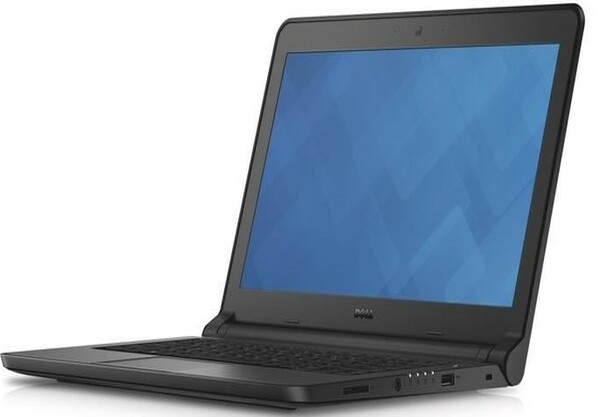
\includegraphics[scale=0.4]{Ressources/Materiel/L3340.jpg}\vspace{-2cm}
\end{wrapfigure}
\paragraph{}\textbf{Dell Latitude 3340 :} \\
\begin{itemize}
\item \textbf{CPU :} Intel Core i5-4210U
\item \textbf{RAM :} 8 Go
\item \textbf{OS :} Windows 10
\item \textbf{Disque Dur :} 256 Go SSD
\item \textbf{Quantité :} 23 unités
\\ \\ \\ \\
\end{itemize}
%%%%%%%%%%%%%%%
\begin{wrapfigure}{c}{7cm}
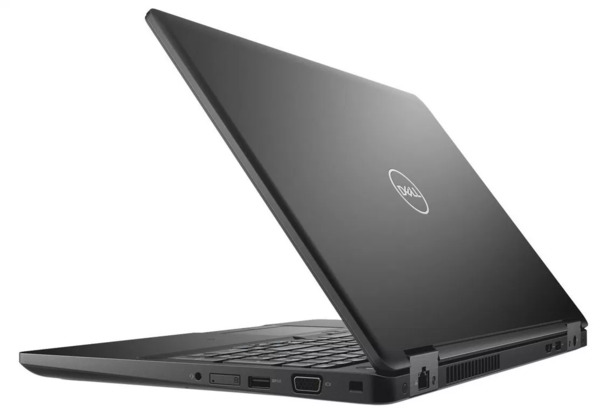
\includegraphics[scale=0.35]{Ressources/Materiel/L5591.jpg}\vspace{-2cm}
\end{wrapfigure}
\paragraph{}\textbf{Dell Latitude 5591 :} \\
\begin{itemize}
\item \textbf{CPU :} Intel Core i5-4210U
\item \textbf{RAM :} 8 Go
\item \textbf{OS :} Windows 10
\item \textbf{Disque Dur :} 256 Go SSD
\item \textbf{Quantité :} 14 unités
\\ \\ \\ \\
\end{itemize}
%%%%%%%%%%%%%%%
\begin{wrapfigure}{c}{7cm}
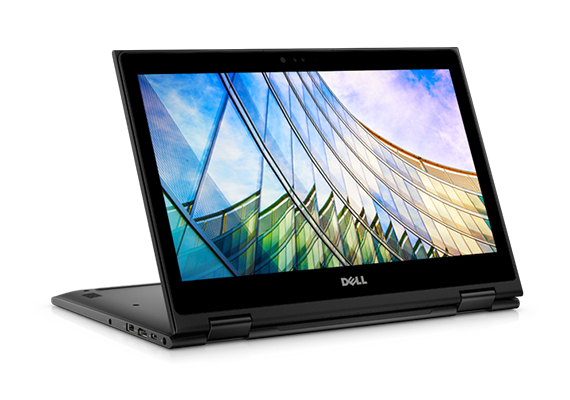
\includegraphics[scale=0.35]{Ressources/Materiel/3390.png}\vspace{-2cm}
\end{wrapfigure}
\paragraph{}\textbf{Dell Latitude 3390 2-in-1 :} \\
\begin{itemize}
\item \textbf{CPU :} Intel Core i5-8250U
\item \textbf{RAM :} 16 Go
\item \textbf{OS :} Windows 10
\item \textbf{Disque Dur :} 256 Go SSD
\item \textbf{Quantité :} 4 unités
\\ \\ \\ \\
\end{itemize}

% ##### Page 6 #####
\newpage
\section{Objectif(s) du stage}

Lors du 1\ier{} entretien effectué chez POLYSOUDE, le responsable informatique recherchait une personne autonome, réactive, diplomate (en fonction des situations et des demande) et capable de travailler en équipe afin d’assurer le support de l’ensemble du parc informatique.\\

Cela était pour moi la 1\ier{} fois que ce type de mission et de telles responsabilités m’étaient confiées au sein d’un parc de plus de 150 postes et surtout au sein d’une équipe.\\

Les tâches qui m’ont été confiées au fil du temps furent : \\
\begin{itemize}
    \item Répondre aux appels téléphoniques du Helpdesk pour une intervention par téléphone ou sur site.
    \item Ouvrir des tickets de support chez nos différents prestataires (téléphonie, infra, applications métiers…).
    \item Gestion des demandes et des incidents (logiciels et matériels) via l’outil GLPI.
    \item Former les utilisateurs sur les outils / matériels mis à disposition.
    \item Ré-initialisation des mots de passe et déverrouillage des comptes des     utilisateurs.
    \item Mise en place et suivi de la gestion de parc.
    \item Remise en norme du câblage électrique/informatique des bureaux (Suivi CHSCT). 
    \item Ergonomie, travail sur écrans. Installation de matériels adaptés et accompagnement des utilisateurs sur les gestes et postures à adopter. 
    \item Déploiement de postes.
    \item Suivi et amélioration du master Polysoude via MDT.
    \item Mise en place d’un serveur de déploiement automatisé.

\end{itemize}

% ##### Page 7 ######
\newpage
\section{Environnement du stage}

L'entreprise comporte 2 niveaux et chaque niveau est découpée en plusieurs zones et/ou service.

Le fait que l'entreprise soit découpé en plusieurs zones, il y a des contraintes liées à la sécurité de l'employé. Un marquage au sol est présent et ainsi soumis à des règles de sécurité tel que le port des \textbf{EPI}\footnote{Equipement de Portection Individuelle}.

Lorsque d'une demande d'intervention est déclenchée, nous veillons à respecter les règles de sécurité mise en \oe{}uvre pour notre propre sécurité et aussi celles des autres collaborateurs.\\
\begin{itemize}
    \item \textbf{Bande jaune :} Port des \textbf{chaussures de sécurité}
    \item \textbf{Bande rouge :} Port de tous les \textbf{EPI} (Casque, Lunette, Chaussure de sécurité)
\end{itemize}

\begin{center}
    \textbf{N.B :} Les \textbf{EPI} répondent à la norme \textbf{ISO 13.340\footnote{https://www.iso.org}}
\end{center}

L'encadrement du service informatique est assez large car nous avons eu à répondre à des incidents liés aux filiales étrangères de Polysoude...

\begin{itemize}
    \item Support mail en Anglais
    \item Support vocal en Anglais \\
\end{itemize}

... Mais aussi avec les intervenants externes (collaborateurs étrangers, clients) lors de leurs visites au sein de la société. Cela pouvait être des incidents lambda :

\begin{itemize}
    \item L'accès au réseau Wifi "invité"
    \item L'utilisation du vidéo-projecteur
    \item Prêt d'un chargeur 
    \item Prêt d'un PC Portable en changeant ou non la langue d'affichage
\end{itemize}

Ces multiples tâches sont effectuées au quotidien au sein du service en parallèle des projets informatiques tel que :

\begin{itemize}
    \item Migration du parc informatique
    \item Formation auprès des utilisateurs
    \item Installation d'éléments dit "ergonomique" (bras écran, support de PC, rehausseur d'écran) 
    \item Création des nouveaux utilisateurs dans l'AD 
    \item Documentation
\end{itemize}

Nous avons à notre disposition, lorsque que nous traitons des demandes/incidents :

\begin{itemize}
    \item Brainstorming, c'est-à-dire l'échange avec les membres de l'équipe IT
    \item Poste Informatique "personnel"
    \item Logithèque
    \item Base de connaissance sous GLPI
    \item Archive mail
    \item Connexion VPN
    \item Accès Internet 
\end{itemize}

% ##### Page 8 ######
\newpage
\section{Présentation des principales activités \& réalisation durant le stage}
\subsection{Support utilisateur}

\begin{figure}[!h]
\centering
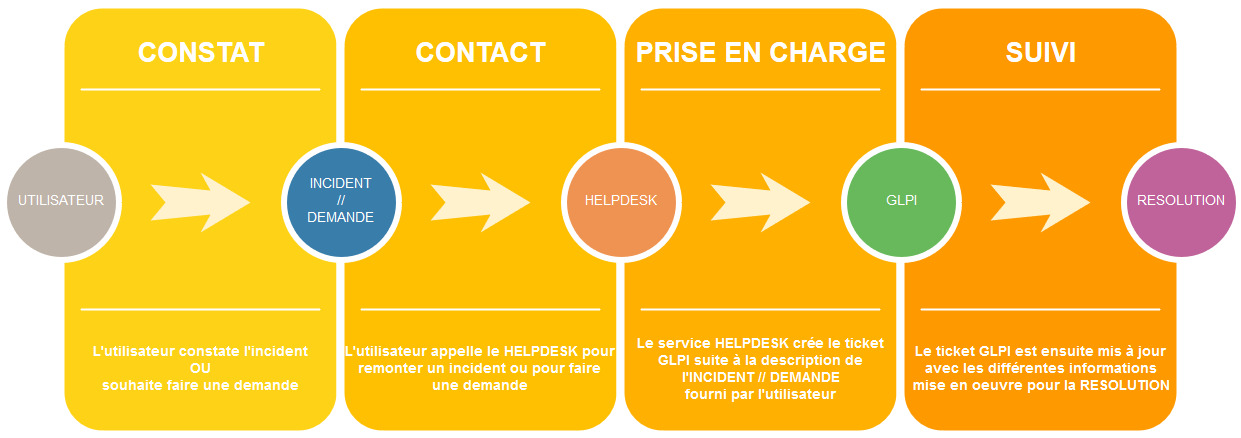
\includegraphics[scale=0.42]{Ressources/GLPI.jpg}
\caption{Schéma de support}
\end{figure}

Dès le besoin d'assistance, les utilisateurs appelant le numéro du \textbf{Helpdesk}. Ce numéro est utilisé par un groupe d'appel géré par \textbf{Shoreware Director}\footnote{Serveur VOIP} pour faire une boucle sur le téléphone de mon collègue ainsi que le mien (DECT ou IPPHONE). \\

En détail du schéma ci-dessus, voici un exemple de notre démarche de support :

\begin{enumerate}
\item \textbf{L'utilisateur} constate qu'il n'arrive pas à ouvrir sa session Windows.
\item Cet utilisateur va appelé le \textbf{Helpdesk} pour avoir l'un des 2 techniciens support et ainsi prend en charge l'incident ou la demande.
\item \textbf{L'un des techniciens support} prend en charge l'appel en posant les bonnes questions (ouvertes ou fermées).
\item Le technicien qui à prit l'appel va ouvrir un ticket sous \textbf{GLPI} en mettant le plus de détails sur l'incident.
\item  Si c'est possible, le technicien va \textbf{intervenir} à distance ou sinon sur site jusqu'à la \textbf{résolution} de l'incident en décrivant toutes les étapes sous le ticket ouvert précedemment.
\end{enumerate}

\newpage

% ##### Page 9 ######
\subsection{Déploiement de poste}
\subsubsection{Idée générale}

Dans le cadre d’une nouvelle installation de Windows 7 ou de Windows 10, nous utilisons un outil de déploiement automatisé appelé \textbf{MDT} \footnote{Microsoft Deployment Toolkit}.
Grâce à cet outil, il est facile de créer son image personnalisée de Windows et de la déployer sur différents postes.

Cela permet d’automatiser l’installation de l’OS ainsi que des logiciels sur un ou plusieurs postes à la fois.
\subsubsection{Préparation post-déploiement}
\begin{enumerate}
    \item \textbf{Les pré-requis :}
\end{enumerate}
•	Un support d’installation (Clé USB, Disque dur externe) bootable ou serveur de déploiement WDS. \\
•	Une connexion filaire. \\
•	Un ordinateur à déployer (PC Portable ou Fixe). \\
•	La roadmap (Feuille de suivi)

\begin{enumerate}
\setcounter{enumi}{1}
    \item \textbf{La roadmap :} \hyperref[sec:Annexes]{Cf.Annexe \no{}2}
\end{enumerate}

•	Les informations de l’utilisateur ainsi que le nom du poste. \\
•	Quel type de système d’exploitation à installer.\\
•	Les diverses étapes de configuration à faire.\\
•	Les logiciels à installer (avec le master et manuellement).\\
•	La configuration du profil utilisateur.\\
•	Et si besoin, une récupération de données à faire (s'il s’agit d’un changement ou d’une réinstallation de poste).

\subsubsection{Processus de déploiement}
En ayant validé toutes les informations « post-déploiement », cela va commercer les différents processus de déploiement en commençant par : \\
\begin{enumerate}
    \item Le formatage et le partitionnement du disque prédéfini dans la console MDT.
    \item L’injection des pilotes : En fonction de la marque et du modèle de l’ordinateur, les pilotes seront copiés et installés.
    \item Installation du système d’exploitation : l’OS est prédéfini depuis la console MDT en utilisant une image « .WIM » fourni avec le CD d’installation ou une image ISO d’installation.
    \item Installation des applications souhaitées : Ces dernières peuvent être installées en bundle.
    \item Scripts de configuration pour divers paramétrages d’utilisation telle que le verrouillage numérique au démarrage, règles de l'ANSSI.
    \item Quelques redémarrages …
    \item … Et une fenêtre montrant si le déploiement s’est bien passé ou s’il y a eu des erreurs.
\end{enumerate}	

\newpage

\section{Conclusion}
Ces différentes expériences et missions m’ont permis d’approfondir et d’intégrer mes connaissances et ma passion pour les nouvelles technologiques au sein d’un environnement professionnel. Cela m’a également permis de développer des qualités relationnels, d’écoute et de communication grâce aux contacts avec les utilisateurs. \\

L’objectif principal de ma démarche est d’élargir mes compétences techniques dans le domaine du support informatique. Les périodes en entreprise m’ont appris de nouvelles méthodes d’organisation. J’ai également gagné en autonomie et surtout en confiance en moi en étant fier des missions, menées à bien, qui m’avaient été confiées ! \\

C’est pour cela que je considère la formation de \textbf{Technicien Supérieur de Support en Informatique} au sein de l’ENI comme un choix important pour perfectionner mes méthodologies, mes compétences ainsi que mon sens des responsabilités.
\newpage

\section{Annexes}
\label{sec:Annexes}
\subsection{Annexe 1 : Infra}
\rotatebox{90}{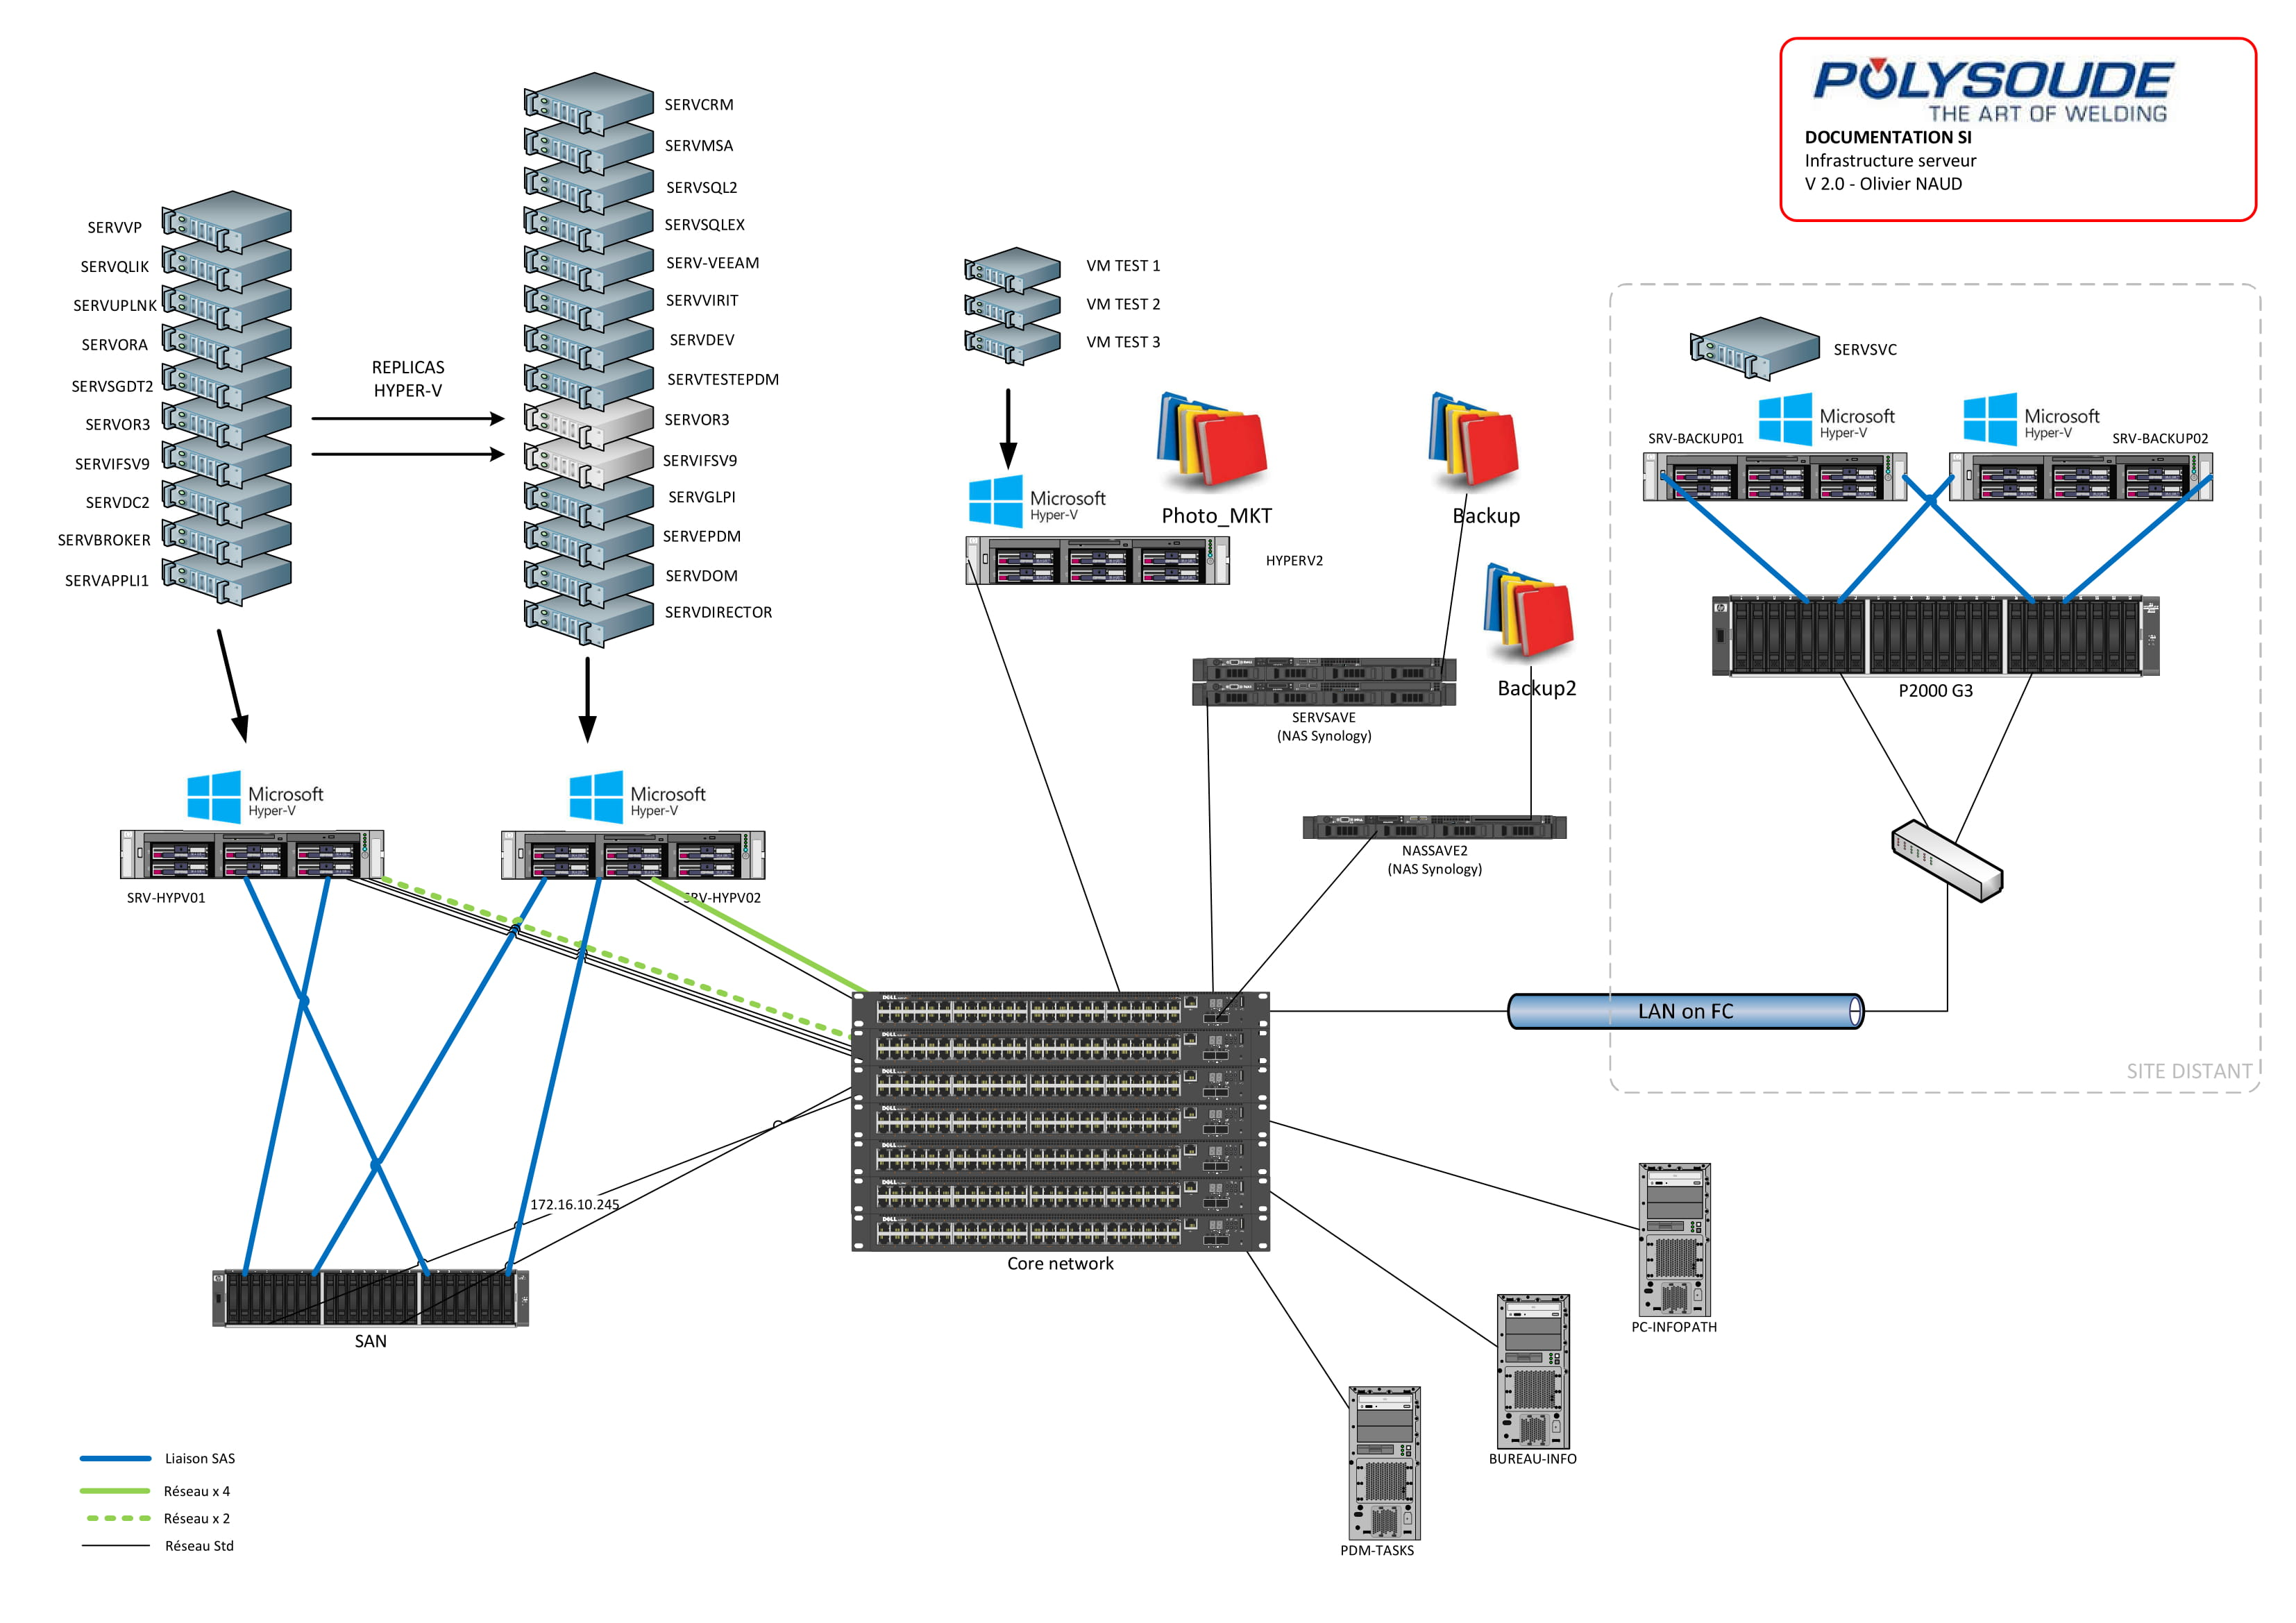
\includegraphics[scale=0.2]{Ressources/Reseau.jpg}}

\subsection{Annexe 2 : La Roadmap}
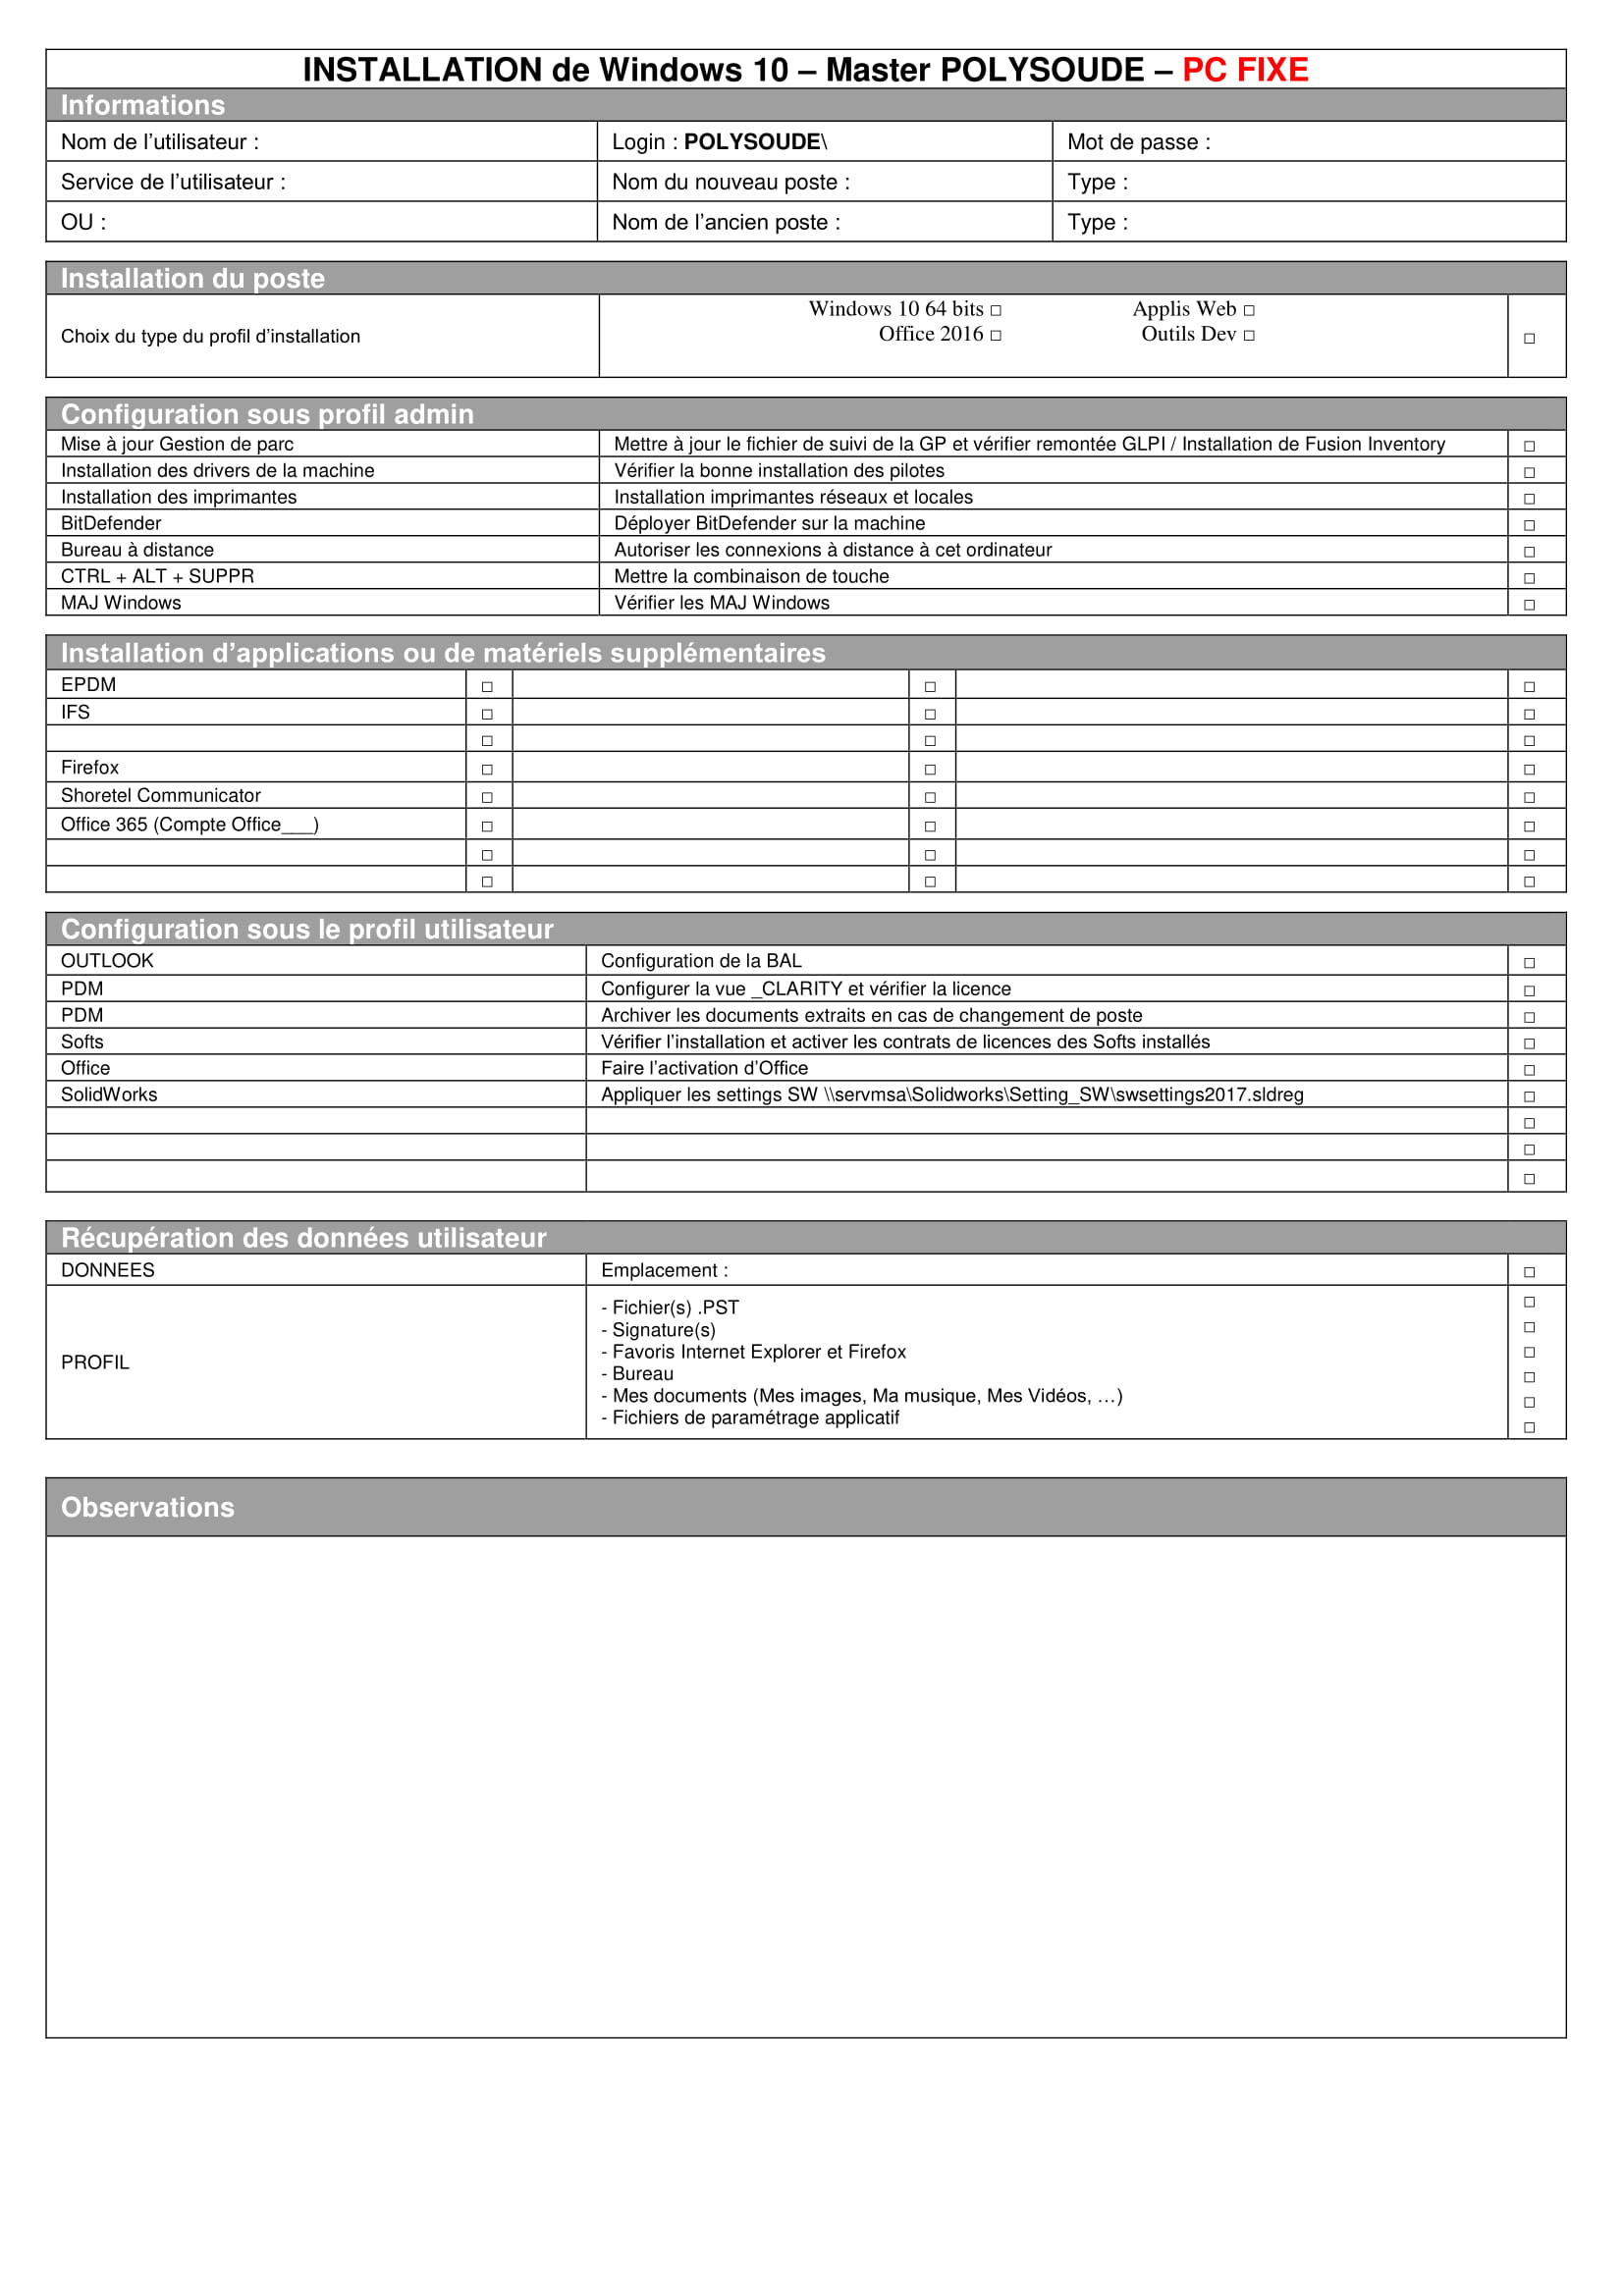
\includegraphics[width=\textwidth]{Ressources/Roadmap.jpg}
\end{document}